\chapter{Basics}
\label{CHAPTER:BASICS}

This chapter contains overview of methods and models that we will use in this
thesis. We describe generative probabilistic models called hidden Markov
models, their variants, and algorithms that are used with these models.
Additionally we describe sequence alignment and several applications of hidden
Markov models to sequence alignment and sequence annotation. In this thesis, we
study hidden Markov models from two aspects: computational complexity of some
HMM problems, and application of HMMs to sequence alignment problem.

\section{Hidden Markov Models}
\abbreviation{Hidden Markov Models}{HMM} are graphical probabilistic models
commonly used for sequence annotation or sequence alignment. An HMM is a
probabilistic finite state machine that in every state emits one symbol. Later
we will also discuss variants of HMMs that emit more symbols or that emit
symbols on multiple tapes. This section describes basic definitions
and algorithms that are used with HMMs.

\subsection{Definitions}\label{SECTION:HMMDEF}
                       
HMMs are generative probabilistic models.
The generative process of an HMM starts in a random state $q$ sampled according
to the \firstUseOf{initial
distribution} $I$.  When an HMM is in some state $q$ it emits one symbol from
alphabet $\Sigma$ according distribution $e_q$ and moves to another state
according to transition distribution $a_q$. Note that emission and transition
distributions can be different for every state.  This process produces two
sequences: sequence of states $\pi=\pi_0\pi_1\pi_2\dots$ called
\firstUseOf{state path} and output sequence $X=X_0X_1X_2\dots$ over alphabet
$\Sigma$. In this work, we will use only discrete versions of HMMs with finite state
space and alphabet.  


\begin{definition}
Any square matrix $M$ of size $n\times n$ is \firstUseOf{stochastic} if it satisfies the
following properties.
\begin{enumerate}[itemsep=-1mm]
\item $\forall 0\leq i<n,0\leq j < m, 0\leq M[i,j]\leq 1$
\item $\forall 0\le i<n, \sum_{i=0}^{m-1}M[i,j]=1$
\end{enumerate}
\end{definition}

\begin{note}
Stochastic matrix consists from $n$ probability distributions over a set of size $n$.
\end{note}

\begin{definition}\label{DEF:HMM}
A \abbreviation{Hidden Markov Model}{HMM} is a tuple $H=(\Sigma,V,I,e,a)$ where
$\Sigma=\{\sigma_0,\dots\sigma_{m-1}\}$ is a finite alphabet of size $m$,
$V=\{v_0,\dots,v_{k-1}\}$ is a finite set of state of size $k$, $I$ is
a distribution over $V$, $e$ is $k\times m$ matrix where each row contains
distribution over $\Sigma$ and $a$ is stochastic matrix of size $m\times m$.

We will index elements of $e$ and $a$ by subscripts; therefore $e_{u,v}$ is
the element in $u$-th row and $v$-th column of $e$.  

\end{definition}

\begin{example}\label{EXAMPLE:EXAMPLEHMM} Consider the HMM $H=(\Sigma,V,I,e,a)$ from Figure
\ref{FIGURE:EXAMPLEHMM}.  Alphabet is $\Sigma=\{A,C,G,T\}$ and set of states is
$V=\{R,0,1\}$.  Transition and emission distributions are described in the figure.
We can define initial distribution to $I_R=0.5, I_1=0.3$ and $I_{0}=0.2$.
\end{example}

\begin{figure}
\begin{center}
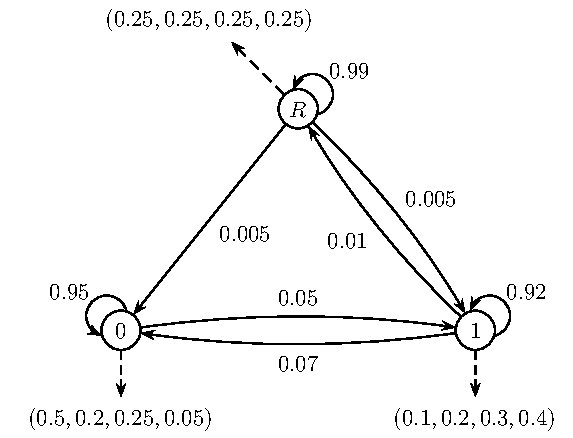
\includegraphics{../figures/exampleHMM.pdf}
\end{center}
\caption[Example of simple Hidden Markov Model]{
An HMM with $3$ states
that emits symbols from alphabet of size $4$.  Circles represents states; an arc
from state $u$ to $v$ indicates that $a_{u,v}>0$. The missing arc from state
$In$ to $R$ means that $a_{In,R}=0$. Every four tuple represents the emission distribution of the associated state.
}\label{FIGURE:EXAMPLEHMM} 
\end{figure}


\begin{definition}\label{DEF:STATEPATH}
Let $H=(\Sigma,V,I,e,a)$ be an HMM. We say that there is \firstUseOf{transition}
from state $u$ to state $v$ if $a_{u,v}>0$. We will write transition from $u$ to
$v$ as $u\to v$ and $T=\{u\to v\mid a_{u,v}>0\}$ is the set of all transitions of
$H$.

\firstUseOf{State path} $\pi=\pi_0\pi_1\dots\pi_{n-1}$ is a sequence of
states. We say that a state path $\pi$ is \firstUseOf{admissible} if $I_{\pi_0}>0$
and  $\pi_{i-1}\to\pi_i\in T$ for all $1\leq i < n$. Otherwise $\pi$ is
\firstUseOf{inadmissible}.
\end{definition}

\begin{example}
Consider the HMM from figure \ref{FIGURE:EXAMPLEHMM}. Set of transitions is
$T=\{R\to R,R\to In, R\to E,In\to In, In\to E, E\to E, E\to In, E\to R\}$.
State path $\pi_1=RRRRInER$ is an admissible state path and $\pi_2=RRRInREER$
is an inadmissible state path, because it contains a transition with zero
probability ($In\to R$).
\end{example}

Hidden Markov models are generative probabilistic models, meaning that they
describe a simple process that can generate a pair of state path and sequence.
In following definition we will define probability distribution of pairs (state
path, sequence) and probability distribution of sequences generated by an HMM.

\begin{definition}
Let $H=(\Sigma,V,I,e,a)$ be an HMM and $X=X_0X_1\dots X_{n-1}$ be a sequence over
alphabet $\Sigma$ of length $n$. Let $\pi$ be a state path of length $n$. Then the
probability that state path $\pi$ generated sequence $X$ is 

\[\prob{X,\pi\mid H}=
I_{\pi_0}e_{\pi_0,X_0}\prod_{i=1}^{|X|-1}a_{\pi_{i-1},\pi_i}e_{\pi_i,X_i}\]
The probability that $X$ was generated by the
model $H$ (using any state path) is 
\[\Pr\left(X\mid H\right)=\sum_{\pi\in V^n}\Pr\left(X,\pi\mid H\right)\]

\end{definition}

\begin{example}
Consider the HMM $H$ from the example \ref{EXAMPLE:EXAMPLEHMM}. Let state path be $\pi=RRInInE$ and
generated sequence be $X=ACGTT$. Then the probability that $H$ generates $\pi$
and $X$ is 
$\prob{ X,\pi\mid H } = 0.5 \cdot 0.35 \cdot 0.99 \cdot 0.25 \cdot 0.005 \cdot 0.25 \cdot 0.95 \cdot 0.05 \cdot 0.05 \cdot 0.4 =
0.5143359375  \cdot  10^{-7}$
\end{example}



\begin{note}
In our  definition of an HMM, the sum of the probabilities of all sequences of
length $n$ is $1$. Later we will discuss concept of final states. With final
states, the sum of the probabilities of all sequences (of all lengths) is one.

\end{note}

We will be interested in the three basic problems in HMMs:
\begin{enumerate}[itemsep=-1mm]
\item Given sequence $X$ and model $H$. What is the probability that $X$ was
generated by model $H$?
\item Given sequence $X$, model $H$ and assumption that $X$ was generated by the
model
$H$, what is the best explanation of $X$? By explanation is usually meant state
path that generated $X$. We call the process of computing explanation of
sequence $X$ \firstUseOf{decoding}.
\item Given training data $D$ (usually sequences with ``explanations'') and
topology of the model (set of states and transitions), what are the best parameters
(initial, transition and emission distributions) that explains training
data $D$? This problem is also called \firstUseOf{training}
\end{enumerate} 
In following sections we will discuss several algorithms
for the problems describes above. We will mostly focus on the
decoding problem.


\subsection{The Forward Algorithm}
The Forward algorithm computes for a given sequence $X$ of
length $n$ the probability $\Pr\left(X\mid H\right)$ that the sequence was
generated by the model (it solves the first problem of HMMs) \cite{Durbin1998}. The algorithm is
based on the dynamic programming. It fills
matrix $F$ of size $n\times m$ where $m$ is the number of states of $H$, $F[i,v]$ is the probability that $H$
generated $X[:i+1]$ with state path that ends in state $v$. Values $F[i,v]$ are  called \firstUseOf{forward
variables}. $F[i,v]$ can be computed by the following equations (also called the
forward equations).

\begin{align}
F[0,v] &= I_ve_{v,X_0}, v\in V\\
F[i,v] &= \sum_{u\in V}F[i-1,u] \cdot a_{u,v} \cdot e_{v,X_i}, v\in V,0< i < n
\end{align}
The probability that $H$ generated $X$ is 
 \[\Pr\left(X\mid H\right) = \sum_{v\in V} F[n-1,v]\]

Using the recurrence equations above, we can compute the probability of $X$ in
$O(nm^2)$ time and $O(m)$ memory. If the transition
matrix is sparse, then this algorithm can be implemented in $O(n(m+t))$ time
where $t$ is the number of transitions.  Forward variables are also used in other
algorithms. 

\subsection{The Viterbi Algorithm}\label{SECTION:VITERBI}
The Viterbi algorithm  is probably the most frequently used
decoding algorithm for hidden Markov
models \cite{Durbin1998}.
The Viterbi algorithm answers a straightforward question: given the sequence
$X=X_0X_1\dots X_{n-1}$, what
is the most-likely state path $\pi$ that generates $X$? Formally, Viterbi
algorithm finds a state path maximizing $\Pr\left( \pi\mid X,H \right)$. Since
\[\Pr\left(\pi\mid X,H\right) = \frac{\Pr\left(\pi,X,\mid
H\right)}{\Pr\left(X\mid H\right)}\] and quantity $\Pr\left(X\mid H\right)$ is
fixed, the most probable state path $\pi$ also maximizes $\Pr\left(X,\pi\mid H\right)$. 

The Viterbi algorithm is very similar to the  Forward algorithm. It starts with computing
Viterbi variables $V[i,v]$. Variable $V[i,v]$ stores the probability of the most probable 
state path that generated $X[:i+1]$ and ends in state $v$. The algorithm
also computes back-links $B[i,v]$ that contain the previous state in the most
probable state path that generated $X[:i+1]$ and ends in state $v$. We can
compute these values by the following equations (called the Viterbi equations):
\begin{align}
V[0,v] &= I_{v}e_{v,X_0}, v\in V\\
V[i,v] &= \max_{u\in V} V[i-1,u]a_{u,v}e_{v,X_i}, v\in V,0<i<n\\
B[i,v] &= \arg\max_{u\in V} V[i-1,u]a_{u,v}e_{v,X_i}, v\in V,0<i<n
\end{align}
\begin{note}
Values $B[0,v],v\in V$ are not needed in the algorithm.

Note the similarity of the Viterbi algorithm and the Forward algorithm.
We can obtain the Viterbi equations from the Forward equations by replacing
summation with
maximization.
\end{note}


Variable $V[n-1,v]$ contains the probability of the most probable state path
that generated $X$ and ends in state $v$. Therefore the state $v_{\max} =
\arg\max_{v\in V}V[n-1,v]$ is the last state of the most probable state path.
Variable $B[n-1,v_{\max}]$ contains the previous state of the most probable
state path. By traversing back through back-links $B$ we can reconstruct the most
probable state path in $O(n)$ time.

Time complexity of the Viterbi algorithm is $O(nm^2)$ or $O(n(m+t))$ for sparse
transition matrices ($m$ is the number of states and $t$ is the number of
transitions).

\subsubsection{Implementation of the }

\subsection{The Forward-Backward Algorithm and  the Posterior Decoding}

The \firstUseOf{Posterior decoding} is another commonly used decoding method
\cite{Kall2005, Durbin1998}. In contrast to the Viterbi algorithm, the
Posterior decoding assigns a label individually to every symbol of an input
sequence and does not care about the overall structure of the reconstructed
state path. 

Given sequence $X$, posterior decoding finds state path $\pi$ with the following
property:
\[\forall 0\leq i< n, \pi_i=\arg\max_{v\in V}\Pr\left(\pi_i=v\mid X,H\right) \]
where \[\Pr\left(\pi_i=v\mid X,H\right) = \sum_{\pi\in V^n,\pi_i=v}\Pr\left(\pi\mid X,H\right)\]

Values $\Pr\left(\pi_i=v\mid X,H\right)$ for every
combination of position $i$ and state $v$ can be computed using the Forward-Backward
algorithm. In particular,

\begin{equation}
\Pr\left(\pi_i=v,X\mid H\right) =  F[i,v]B[i, v]
\end{equation}
In this formula, value $B[i, v]$ is defined as 
\begin{equation}
B[i, v] =	
					\sum_{\pi\in V^{n-i},\pi_0=v}
					\prod_{j=1}^{n-i-1} e_{\pi_j,X_{i+j}}a_{\pi_{j-1},\pi_j}
\end{equation}

We can compute 
these values using  the Backward algorithm, which is very similar to the Forward
algorithm. 
\begin{align}
B[i,v]&=
\begin{cases}
1 & \textrm{if $i=n-1$}\\
 \sum_{u\in V}
 	e_{\pi_j,X_{i+1}}a_{v,u}B[i+1,u] & \textrm{otherwise}
\end{cases}
\end{align}

The cell $B[i,v]$ depends on the next positions in sequence $X$,
while $F[i,v]$ depends on the previous positions in sequence $X$. Another
difference is that $B[i,v]$ does include emission of $X[i]$ while $F[i,v]$ does.

We can compute values of $F[i,v]$ and $B[i,v]$ and find the posterior decoding
in $O(n(m+t))$ time and $O(nm)$ memory.  Advantage of posterior decoding is
that it uses information from many slightly suboptimal state paths as opposed
to Viterbi decoding, which uses only one state path. One drawback is that it
can reconstruct inadmissible state path. Example is given below.



\begin{figure}
\begin{center}
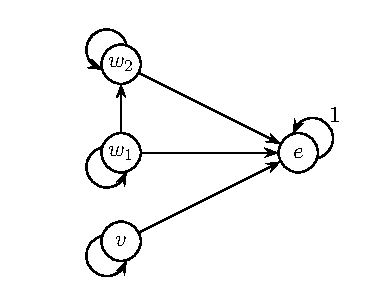
\includegraphics{../figures/posteriorInadmissibleStatePath.pdf}
\end{center}
\caption[Hidden Markov Model on which posterior decoding reconstructs
inadmissible state path]{
Example of an HMM on which the Posterior decoding reconstructs inadmissible state path. 
All unlabeled transitions are even ($0.5$). States $w_1,w_2,$ and $v$ emits $0$
with probability $1$ and state $e$ emits $1$ with probability $1$.
Initial distribution is set to $I_{w_1}=I_{w_2}=0.3, I_{v}=0.4, I_{e}=0$.
}\label{FIGURE:INADMISSIBLESTATEPATH}
\end{figure}

\begin{example}
Consider an HMM from figure \ref{FIGURE:INADMISSIBLESTATEPATH}. Let $X=001$. There
are three state paths that have non-zero probability:
$\pi_1=w_1w_2e,\pi_2=w_2w_1e,$ and $\pi_3=vve$. Their probabilities are
$\prob{\pi_1\mid X,H}=\prob{\pi_2\mid X,H}=0.3,$ and $\prob{\pi_3\mid X,H}=0.4$
respectively.
Posterior probabilities are in table \ref{TABLE:INADMISSIBLESTATEPATH}.
As we can see, the maximal posterior probability for the first position has state
$v$. For the second position it is state $w_2$ and for the third it is state
$e$. Therefore PD will reconstruct state path $vw_2e$. However, this state path 
is inadmissible since  $v\to w_2$ is not a transition (it has zero probability).

\begin{table}
\begin{center}
\begin{tabular}{|l|c|c|c|}
\hline
State/Position & $X_0$ & $X_1$ & $X_2$ \\\hline
$w_1$ & $0.3$ & $0$ & $0$ \\\hline
$w_2$ & $0.3$ & $0.6$ & $0$ \\\hline
$v$   & $0.4$ & $0.4$ & $0$\\\hline
$e$  & $0$ & $0$ & $1$ \\\hline
\end{tabular}
\end{center}
\caption[Example of posterior probabilities.]{Posterior probabilities for
the sequence $X$ and the HMM $H$ from the figure \ref{FIGURE:INADMISSIBLESTATEPATH}.
}\label{TABLE:INADMISSIBLESTATEPATH}
\end{table}

\end{example}

\subsection{Sequence Annotation}


HMMs can be used for sequence annotation. By sequence annotation we mean
assigning ``labels'' to parts of the input sequence according to their meaning.
So far we have described two algorithms that can be used for sequence
annotation: the Viterbi algorithm and the Posterior decoding. In both
algorithms, the sequence annotation is the output from the algorithm: the
decoded state path. Now we give several examples of bioinformatics problems
where HMMs were previously used. 

\paragraph{Gene finding:} Parts of DNA sequences that are in cells translated
into proteins are called genes.  In gene finding we want to assign to every
symbol of the input sequence a gene label if it is inside a gene or a different
label if it is not part of a gene \cite{GeneWise2004, Brejova2005, Burge1997,
Alexanderson2004}. Additionally, we want to label sequence according to the
internal structure of a gene: gene starts with promoter followed by
transcription start site and ends with transcription stop site. Between
transcription sites are alternating exons and introns \cite{TODO}. 


\paragraph{Transmembrane proteins:} Some proteins in cells pass through a membrane
from one side to the another (usually they pass through the membrane several times).  In
transmembrane protein prediction we want to assign labels to the symbols of the input
protein sequence to distinguish the parts of the sequence that are on one side of the
membrane from the parts that are on the other side of membrane or inside the membrane
\cite{Brown2010}.

\paragraph{Recombination prediction:} Some organisms, for example HIV virus,
evolve rapidly and have been classified into several subtypes.  Moreover,
some viruses are mosaic combination of viruses from different subtypes. For
example, beginning and end of the sequence of a virus can be from one subtype and
the middle of the sequence is from a different subtype. In recombination prediction,
we want to annotate the sequence to distinguish between parts that originate in
different subtypes \cite{Nanasi2010,Truszkowski2011}.  

\paragraph{} In general,
we have a finite set of labels $C=\{c_0,c_1,\dots,c_{l-1}\}$ and we want to
assign one label to every symbol of the input sequence. We do it by assigning
one label to every state of an HMM.
To predict the annotation of the input sequence $X$, we can  find the
most probable state path that could generate $X$ and  annotate each symbol of
the sequence $X$ according to the label assigned to the state that generated that
symbol. We can formalize it in the following definition.

\begin{definition}\label{DEFINITION:ANNOTATION}
Let $H=(\Sigma,V,I,e,a)$ be HMM and $C=\{c_0,c_1,\dots,c_{l-1}\}$ be the finite
sets of labels (or colors). Then the \firstUseOf{coloring function} 
$\lambda: V^*\to C^*$ is function that satisfies following properties:
\begin{enumerate}[itemsep=-1mm]
\item $\lambda(v)\in C$ for all $v\in V$.
\item $\lambda(xy) = \lambda(x)\lambda(y)$ for all $x,y\in V^*$.
\end{enumerate}

Let $X$ be a sequence generated by state path $\pi$. Then annotation
$\Lambda$ of sequence $X$ is $\Lambda = \lambda(\pi)$.
\end{definition}

In the sequence annotation problem, we do not know the state path $\pi$ that
generated a given sequence. Our goal is to reconstruct the state path $\pi$ or
at least to give a good approximation of the correct annotation $\Lambda(\pi)$.
Note that in general, several state paths can have the same label.

\begin{definition}
Let $H$ be an $HMM$, $X$ be a sequence of length $n$, $\Lambda$ be an annotation of sequence
$X$. The probability of annotation $\Lambda$ given sequence $X$ is 
\begin{equation}
\Pr\left(\Lambda\mid X,H\right)=\sum_{\pi \in V^n,\lambda(\pi) =
\Lambda}\Pr\left(\pi\mid X,H \right)\label{DEF:ANNOTATION:PROBABILITY}
\end{equation}
\end{definition}

Note that $\prob{\pi\mid X,H}=\frac{\prob{\pi,X\mid H}}{\prob{X\mid
H}}$.

\begin{example}\label{EXAMPLE:ANNOTATION}
Let $H$ be the HMM from the example \ref{EXAMPLE:EXAMPLEHMM}. Let $C=\{I,G\}$ and
$\lambda(R)=I$ and $\lambda(0)=\lambda(1)=G$.  Consider sequence
$X=AACT$, which was generated by the state path $\pi=R011$. The correct
annotation of $X$ is therefore  $\lambda(R011) =
IGGG$. 

 We can imagine $H$ as very simple (and not very realistic) gene
predictor. $R$ represents intergenic regions, state $In$
represents introns and $E$ represents exons. Label $I$ represents
intergenic regions and label $G$ represents regions that are genes.

Using this interpretation, the sequence $AACT$ contains gene $ACT$. There are
several state paths consistent with this annotation: if $AACT$ was generated by state path
$REEE$ then subsequence $EEE$ is exon; if it was generated by state path $REIE$
then sequence contain two exons and one intron in the middle. There are $2^3$
different state paths $\pi$ with $\lambda(\pi)=IGGG$.  All of those state path
support ``fact'' that $IGGG$ is the correct annotation of $X$.

\end{example}

Given a sequence $X$, the natural question is what is the best annotation of
$X$.  One measure of quality of an annotation is its probability. The more
probable is annotation, the more likely $X$ was generated with some state path with
such annotation. We can formulate this in following problem.

\begin{definition}
Given HMM $H$ and sequence $X$, \abbreviation{the most probable annotation
problem}{MPA} is the problem of finding an annotation $\Lambda$ of $X$ that maximizes
the probability \[\prob{\Lambda\mid X,H}\]
\end{definition}

\begin{theorem}
Most probable annotation problem is NP-hard.
\end{theorem}
This theorem was proved in 2002 by Lyngsø {\it et al.} and proof can be found in
\cite{Lyngso2002}. Their proof was done by a reduction from the maximum clique problem.
For input graph with $n$ vertices they construct an HMM $H$ with $O(n^2)$ states and
sequence $X$ of the length $n$. The most probable annotation of $X$ could be
converted into maximum clique of input graph. 
Their result was later strengthened in a sense that the problen is hard even for some constant-sized HMMs \cite{Brejova2007mpa}.

\begin{theorem}
There exists an HMM such that it is NP-hard to find the most probable annotation
to a given input sequence $X$.
\end{theorem}

Same paper also contain polynomial Viterbi-like algorithm (Extended Viterbi
Algorithm) that finds most probable annotation for special classes of HMMs. 

Traditional way to find sequence annotation is to use Viterbi algorithm: given
sequence $X$, we find the most probable state path $\pi$ and then compute
$\lambda(\pi)$. If the  coloring function $\lambda$ is the identity function,
this will find the most probable annotation. In general, the Viterbi
algorithm is not even a good approximation of the most probable annotation as
shown in the following example.

\begin{figure}
\begin{center}
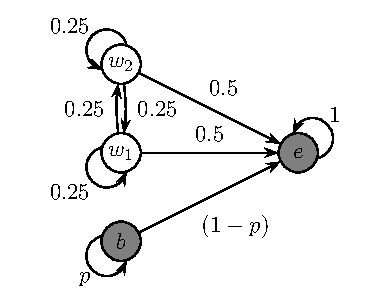
\includegraphics{../figures/multiplePathProblemHMM.pdf}
\end{center}
\caption[Hidden Markov Model with multiple path problem.]{Example of an HMM with
multiple path problem. States $w_1,w_2,b$ emit symbol $0$ with probability $1$
and state $e$ emits symbol $1$ with probability $1$. Initial distribution is set
to $I_{w_1}=I_{w_2}=\frac14, I_{b}=0.5$
and $I_e=0$. Annotations of the states are represented by the colors of the states
($\lambda(w_1)=\lambda(w_2)$ and $\lambda(b)=\lambda(e)$). }\label{FIGURE:BADVITERBIEXAMPLE}
\end{figure}

\begin{example} 
Consider the HMM from Figure \ref{FIGURE:BADVITERBIEXAMPLE}. Take sequence
$X=0^n1$.  Since state $e$ is the only state that can emit $1$, every state
path with non-zero probability ends in state $e$. If a state path starts in
state $b$ then state path has form $b^ne$. Annotation of such a state path is
$\Lambda_1=\lambda(b)^{n+1}$ and probability of the annotation $\Lambda_1$ (and
also the state path $b^ne$) is $p^n(1-p)$.  If a state path starts in the one
of the white states, then a state path has form $w'_0w'_1\dots w'_{n-1}e$ where
$w'_i$ is either $w_1$ or $w_2$.  There are $2^n$ such state paths and each of
them has probability $0.5\cdot 0.25^n$ and annotation
$\Lambda_2=\lambda(w_1)^n\lambda(e)$. Probability of annotation $\Lambda_2$ is
therefore $0.5^{n+1}$.  If $n$ is sufficiently high and $\frac14<p<\frac12$
then the most probable state path is $b^ne$ which corresponds to the annotation
$\Lambda_1$. However, the most probable annotation is $\Lambda_2$ and its
probability is exponentially higher then the probability of $\Lambda_1$.
Therefore the Viterbi algorithm it not even a good approximation of the most
probable annotation problem.

We say that an HMM has the \firstUseOf{multiple path problem} if it has an
annotation that corresponds to more than one state path.
\end{example}


Note that from the probabilistic nature of the HMMs, the most probable
annotation does not have to be the best approximation of the correct annotation.
We will discuss alternative decoding criteria in section \ref{TODO}.
\nocite{Brown2010,Gross2007,Nanasi2010,Truszkowski2011}.


\subsection{Training} 

Training is the process of estimating parameters of the probabilistic models. In this
section we briefly describe several approaches for estimating transition and
emission distributions of hidden Markov models.

We use the \firstUseOf{maximum likelihood approach}. Let $H_{\theta}$ be an HMM
where $\theta$ contains emission and transition probabilities and
let $D$ be training data (the set of pairs $(X,\pi)$ where $X$ is sequence and $\pi$ is a state path).  We
want to find $\theta$ that maximizes the likelihood of the data:

\[L(H_\theta\mid D)=\prob{D\mid H_\theta}= \prod_{(X,\pi)\in D}\prob{X,\pi\mid H_\theta}\]

Under this scenario, we can use the frequencies of occurred events as the parameters of the model \cite{Durbin1998}.
Let $A_{u,v}$ be the number of transitions from $u$ to $v$ in $D$.
Let $E_{u,x}$ be the number times when state $u$ emitted $x$ in training data
$D$.
Then 
\begin{align*}
&a_{u,v}=\frac{A_{u,v}}{\sum_{w\in V}A_{u,w}}
&e_{u,x}=\frac{E_{u,x}}{\sum_{y\in\Sigma}E_{y,x}}
\end{align*}
for all $u,v\in V, x\in\Sigma$. Parameters $\theta=(e,a)$ maximize the likelihood
\cite{Durbin1998}. If case of insufficient data, some events that have
nonzero probability may not occur in the data and therefore their probability will be
estimated to zero. To avoid this behavior, we can use pseudo-counts
\cite{Durbin1998}: we artificially add a constant $k_x$ to the counts of all
events $x$ that we expect to have non-zero probability.

\subsubsection{Training with Missing Data} 
In case that some data are missing (for example a part
of the state path or part of the sequence) we treat the missing data as random
variables. We can use the following algorithm. 
\begin{enumerate}[itemsep=-1mm]
\item  Set the initial parameters $\theta_0$. Let $i=0$
\item  Using model $H_{\theta_i}$, compute the expected number of occurrences of
all events (the values $A_{u,v}, E_{u,x}, u,v\in V,x\in\Sigma$). Compute the new
parameter set $\theta_{i+1}$ from the expected counts (using the method
described above). Set $i=i+1$.
\item If stopping criterion was not reached, go to step two. Otherwise 
set the $H_{\theta_{i}}$ as the final model.
\end{enumerate}
This algorithm is called the Baum-Welch algorithm and it is an instance of the
more general Expectation maximization algorithm \cite{Durbin1998}. Sequence $\{L(H_{\theta_i}\mid D)\}_{i\geq 0}$ is non-decreasing and
 converges to a local minimum \cite{Durbin1998}. As a stopping criterion,
we can use the number of iterations or the change in the likelihood.
 The expectations of the number of events can be
computed by a variant of the Forward-Backward algorithm.

In step $2$ we can replace the Forward-Backward algorithm with the Viterbi
algorithm. In such case the Viterbi algorithm computes the most probable values
for the missing data and new model is estimated from this data.
This approach is called the Viterbi training.  While the Viterbi training does
not have to converge to local maxima, it is faster in practice
\cite{Durbin1998}.  In practice we can use the Viterbi training for the
estimation of good starting parameters for the Baum-Welsch training. The
approach was used in \cite{FEAST2011}.

\subsection{Variants of Hidden Markov Models}

In this section we describe several variants of hidden Markov models.  Some of
these extensions have more expressive power but mostly they are introduced for
simplifying  models. We will use all the described variants later in the
thesis.

\subsubsection{Silent states}
\label{SECTION:SILENT}
One common variant of HMMs are HMMs with silent states. A silent state is a state
that does not emit any symbol. In the presence of silent states a state path can
be longer than the emitted sequence. However, the number of non-silent states in
the state path has to be equal to the sequence length. Silent states do not
add any expressive power to HMMs, but in some cases they allow to reduce the
number of transitions by a factor $m$. This can be used to decrease the number of
parameters and speed up algorithms. 

\begin{figure}
\begin{center}
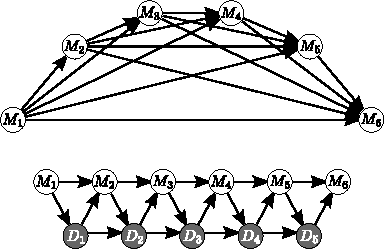
\includegraphics[width=10cm]{../figures/silent_removal.pdf}
\end{center}
\caption[Removal of silent state]{
Upper model without silent states, lower model has silent states $D_1, \dots, D_5$ to simplify 
transitions between states $M_i, 1\leq i\leq 6$.
}\label{FIGURE:SILENTREMOVE}
\end{figure}

\begin{example}
Example of an HMM with silent states that reduces the number of transitions by factor
of $\Theta(m)$.

Consider following HMM $H=(\Sigma,V,I,e,a)$ with $m$ states $M_1,\dots, M_m$
there is transitions from $M_i$ to $M_j$ if and only if $i<j$. Example of such
HMM is in Figure \ref{FIGURE:SILENTREMOVE} and it has in general
$\frac{(m-1)(m-2)}{2}$ transitions.

To reduce number of transitions, we can create HMM $H'=(\Sigma, V', I', e', a')$ by removing all
transitions and  adding chain of delete states $D_1,\dots, D_{m-1}$ with
following transitions: $M_i\to M_{i+1}, M_{i}\to D_{i}, D_{i}]\to M_{i+1}$ for
all $1\leq i<m$ and $D_{i}\to D_{i+1}$ for all $1\leq i<m-1$. Structure of $H'$
is in lower part of Figure \ref{FIGURE:SILENTREMOVE}. We have changed the
number of transitions to $4m-5$ at expense of additional $m-1$ states. In case
of sufficiently large $m$ (at least $12$), $H'$ is smaller. 

Problem is that for certain transition matrices $a$, it is not possible to find
transition matrix $a'$ such that the distributions of sequences of HMM $H$ will
be the same as the distribution of sequences of HMM $H'$. However, this type of
reduction is used in often in practice, for example in profile HMM
\cite{Durbin1998} which are later explained in section \ref{HERD:METHODS}.

The Viterbi algorithm, the Forward algorithm or Posterior decoding can be
implemented for $H'$ in $O(nm)$ time while these algorithm will have time
complexity $O(nm^2)$ for $H$.
\end{example}

There should not be the cycle from transitions between silent states, because
it causes problems with the order of computations of the Viterbi algorithm, the
Forward algorithm and others. For example if we have silent cycle out of states
$u$ and $v$, the recurrency for computing the Forward algorithm contain a
cycle: value $F[i, v]$ depends on value $F[i, u]$, and value $F[i,u]$ depends
on value $F[i, v]$.  Such cycles can be removed from an HMM without affecting
of the distribution of the sequence, and for every HMM with silent
states there is an HMM without silent states that defines same distribution of
sequences \cite{Nanasi2010mgr}.


\subsubsection{Start and Final state}

Sometimes it is useful to have a special start state and a special final state.
Start states can be used instead of the initial distribution. State $s$ is a start
state, if $I_v=1$. Conversely, we can model arbitrary initial distribution by a silent start state $s$
with $a_{s,v}=I_v$ for all $v$.

In contrast, final states affect distribution of the model. An HMM defined in section
\ref{SECTION:HMMDEF} defines a distribution over the sequences of the same length.
An HMM with
final states defines distribution over sequences of all lengths.  We denote the
set of final states $F\subseteq V$. Transitions from final states are not
defined (or set to zero). Emission distribution might be defined (if not, final
states are silent). Every state path has to end with a final state, and
final state can be only at the end of a state path.

With final states, HMM stops generating a sequence once it reaches some final
state. Therefore the sum of the probabilities of all sequences is $1$.

Final states slightly affect algorithms. For example in the Forward algorithm
we do not have to change recurrences, only the final summation: probability of
the sequence is $\sum_{q\in F}F[n-1,q]$.  Similarly, in the Viterbi algorithm
we have to find $\max_{q\in F} V[n-1,q]$ not $\max_{q\in V} V[n-1,q]$.  The
Backward algorithm is changed by setting $B[n-1,q]$ to zero for all $q\notin
F$.

Advantage of start and final states is, that it is trivial to compose model
together.  For example to chain two model, we just merge start state of one
state with final state of other state.

\subsubsection{High Order HMMs}

Sequence $X$ and a state path $\pi$ generated by an HMM can by considered as
sequences of random variables $X_0,X_1,\dots, X_{n-1}$ and
$\pi_0,\pi_1,\dots,\pi_{n-1}$.  Random variables associated with the state path
have the Markov property \cite{Levin2006}, which means that $\pi_i$ depends
only on $\pi_{i-1}$ or more precisely
$\prob{\pi_i\mid\pi_0,\dots,\pi_{i-1}}=\prob{\pi_i\mid\pi_{i-1}}$. Similarly,
$X_i$ depends only on $\pi_i$, that is
$\prob{X_i\mid\pi_0,\dots,\pi_i,X_0,\dots,X_{i-1}}=\prob{X_i\mid\pi_i}$.
However, sometimes the  ability to look back more than just one state or symbol
is useful. We can extend the transition and the emission probabilities to
depend on several previous states/emissions. 

\nocite{Brejova2005,Alexanderson2004}
We will briefly discuss $k$-th order HMMs where emissions are dependent on
previous $k$ emissions. Specifically, $X_i$ depends only on $\pi_i$ and
$X_{i-k},\dots,X_{i-1}$. Emission distribution is therefore parametrized by
state and previous emissions, which is a string of length at most $k$ (it can be
shorter in the beginning of the sequence). $e_{u,x,a}$ is probability that
state $u$ emits $a$ under the condition that $x$ is the suffix of the already emitted
sequence. Let $X$ be sequence and $\pi$ be state path. Then definition
of probability that $X$ and $\pi$ were generated by the model changes to

\[
\prob{X,\pi\mid H} = 
I_{\pi_0}e_{\pi,\varepsilon,X_0}\prod_{i=1}^{n-1}
e_{\pi_i,X[i-\min\{k,i\}:i],X_i}a_{\pi_{i-1},\pi_i}
\]
where $\varepsilon$ is empty string. Other definitions will not change. We can
use all algorithms that we have described above, but we have incorporate these
new emission distributions.

\subsubsection{Generalized HMMs}

Consider a state $v$ with a self-transition, i.e. a state for which $e_{v,v}>0$.
The number of steps the model remains in this state is distributed according to
the geometric distribution.
In particular, the probability that we will leave state $v$ after exactly $k$ steps is
$e_{v,v}^{k-1}(1-e_{v,v})$. For some
applications this behaviour not
appropriate \cite{Burge1997,Majoros2004}.

A \abbreviation{generalized hidden Markov model}{GHMM} (or hidden semi-Markov model)
has with every state $v$ associated a duration distribution $d_v$.  When
a GHMM enters state $v$, it first samples length $l$ according
to the distribution $d_v$.  Afterwards it generates string $x$ of length $l$.  To
specify the probability $e_{v,x}$, each symbol of generated string $x$ is usually
generated independently, which means that $e_{v,x}=\prod_{i=0}^{|x|-1}e_{v,x[i]}$.
Output of a GHMM are three sequences: state path $\pi=\pi_0\pi_1\dots\pi_{l-1}$,
\firstUseOf{duration sequence} $D=D_0D_1\dots D_{l-1}$ and sequence
$X=X_0X_1\dots X_{n-1}$.  The state path and the duration sequence has same
length and \[\sum_{i=0}^{|D|-1}D_i = |X|\].

Manipulation with GHMMs is  more complicated and technical.
Computing this probability of sequence $X$ can be done by a variant of the
Forward algorithm. Finding $\pi$ and $D$ maximizing the probability
$\prob{\pi,D,X\mid H}$ can be found by the variant of the Viterbi algorithm.
However, time complexity of those algorithm on GHMM is higher because for
computing probability $V[i, v]$ (the probability of the most probable state
path ending in state $v$ at position $i$) we have to consider all possible
emission lengths of state $v$, which is $i$. The Viterbi algorithm and the
Forward algorithm run in $O(n^2m^2)$ time.


\section{Other Decoding Methods for HMMs}
In the previous sections we have described two decoding algorithms: the Viterbi algorithm
that finds the most probable state path  and the Posterior decoding that for
every symbol of the sequence assigns the state that generated such symbol with
maximum probability. 
We have shown that in some cases these algorithms can recover bad
annotation. However, maximizing the most probable annotation is NP-hard and
therefore it is not tractable. Additionally, the most probable annotation does
not necessary have to be the best approximation of the true annotation.

In this section we will describe highest expected gain decoding framework,
describe already discussed algorithm within this framework and show several
other decoding methods developed in recent years.

\subsection{Highest Expected Gain}

\label{SECTION:HEG}

In this section we will describe a framework for studying decoding algorithms in
a more systematic way. This framework was introduced  originally for
conditional random fields \cite{Gross2007}.  To use this framework, we need to
define a gain function, which will express similarity (gain) between two
annotations or state paths. The higher the gain, the more similar those two
annotations are. Gain function is domain specific and can penalize the differences
in the domain specific features of the state paths.  Gain function is not a
similarity in the mathematical sense; it does not even have to be symmetric.

Our goal is to find an annotation that is as similar as possible to the correct
annotation. Problem is that we do not know the correct annotation. Our only
assumption is that the input sequence came from the model and therefore we will
treat the correct annotation as a random variable, with probability distribution
defined by the HMM and the observed sequence. We will seek for annotation that
maximizes the highest expected gain \cite{Nanasi2010,Nanasi2010mgr}.

\begin{definition}
Let $H$ be an HMM and $L$ be the set of all annotations. Any function
$f:L\times L\to \mathbb{R}$ is an \firstUseOf{annotation gain function}.

Let $\Pi$ be the set of all state paths. Any function $f:\Pi\times
\Pi\to\mathbb{R}$ is a \firstUseOf{path gain functions}.
\label{DEFINITION:GAINFUNCTION}
\end{definition}

\begin{note}
We will use term gain function instead of annotation/path gain function if it is
clear from the context.

Machine learning literature often uses a related term of loss function
\cite{Lember2010}. Lower loss mean more similar annotations, that is higher gain. Instead
of maximizing the expected gain we can therefore equivalently minimize the expected
loss.
\end{note}

\begin{definition}
Let $H$ be an HMM, $f$ be a gain function, $X$ be a sequence generated by $H$ and
$\Lambda$ be an annotation of $X$. Then the \firstUseOf{expected gain} of annotation
$\Lambda$ is 
\begin{equation}
E_{\Lambda_X\mid X,H}[f(\Lambda_X,\Lambda)] =
\sum_{\Lambda_X}f(\Lambda_X,\Lambda)\Pr\left(\Lambda_X\mid X,H\right)
\end{equation}
Let $\pi$ be a state path. Then the expected gain of state path $\pi$ is 
\begin{equation}
E_{\pi_X\mid X,H}[f(\pi_X,\pi)] =
\sum_{\pi_X}f(\pi_X,\pi)\Pr\left(\pi_X\mid X,H\right)
\end{equation}
\end{definition}


Once we have HMM $H$, gain function $f$ and the observed sequence $X$,
we are trying to find the annotation/state path maximizing the expected gain. 
\begin{equation}
\Lambda = \arg\max_{\Lambda}E_{\Lambda_X\mid
X,H}\left[f\left(\Lambda_x,\Lambda\right)\right]
\end{equation}

We can express the classical decoding algorithms within this framework to show
its universality. We will define two gain functions: $f_A$ which corresponds to
the  
Viterbi algorithm and the most probable annotation problem and $f_p$ which
corresponds to 
the Posterior decoding.

The gain function $f_A$ is simply identity function (definition for state paths
is analogous).
\begin{equation}
f_A(\Lambda,\Lambda') = \begin{cases}
1 & \text{if $\Lambda = \Lambda'$ }\\
0 & \text{if $\Lambda \not=\Lambda'$}
\end{cases}
\end{equation}
For this gain function $E_{\Lambda_X}[f_A(\Lambda_X,\Lambda)]=\prob{\Lambda\mid
X H}$ and this
maximizing expected gain is 
equivalent to the most probable annotation problem. Similarly if we define gain
as the identity function over state paths, we obtain the most probable state
path problem, which can by solved by the Viterbi algorithm.

Therefore for given sequence finding annotation with highest expected gain is
NP-hard if gain function is part of the input. However, for specific gain
functions we can maximize expected gain in polynomial time.

The gain function $f_P$ compares the two annotations of the same length position
by position and assigns score $1$ to every position where they are equal.
\begin{equation}
f_P(\Lambda,\Lambda') = 
\begin{cases}
0 & \text{if $|\Lambda|\not=|\Lambda'|$}\\
\sum_{i=0}^{|\Lambda|-1}\begin{cases}
1 & \text{if $\Lambda_i=\Lambda'_i$}\\
0 & \text{otherwise}
\end{cases}
\end{cases}
\end{equation}

Similarly, we can define gain function $f_P$ for state paths. In such case
maximizing the expected gain is equivalent to the Posterior decoding. Highest
expected gain framework give us another interpretation of the scoring function of
the Posterior decoding. Let $\Lambda_X$  have same length as $\Lambda$. From
linearity of the expectation we have \[E_{\Lambda_X}[f_P(\Lambda_X,\Lambda)] =
\sum_{i=0}^{|\Lambda|-1}E_{\Lambda_X[i]}[f_P(\Lambda_X[i],\Lambda[i])]\] We say
that the $i$-th label of $\Lambda$ is correctly predicted if
$f_P(\Lambda_X[i],\Lambda[i])=1$ (which is true if $\Lambda_X[i]=\Lambda[i]$). Therefore  by maximizing $f_P$ we search for
an annotation/state path that maximizes the expected number of correctly
predicted labels/states.

\subsection{Maximum Boundary Accuracy Decoding}

\abbreviation{Maximum boundary accuracy decoding}{MBAD} is used in the gene-finder
CONTRAST \cite{Gross2007}. It
was proposed for \abbreviation{conditional random fields}{CRF}, but since CRF
are similar to HMM, we define it in the terms of HMMs.

This decoding method  maximize the weighted difference between the expected
number of true-positive and false-positive coding region boundaries.

\begin{definition}
Let $\Lambda=\Lambda_0\Lambda_1\dots\Lambda_{n-1}$ be an annotation. A boundary of
annotation $\Lambda$ is every position $i$ where $\Lambda_{i-1}\not=\Lambda_i$. 
\end{definition}

Maximum boundary accuracy decoding has one parameter $\gamma$. Let $B_{\Lambda'}$ be the
set of all boundaries in $\Lambda'$. Then MBAD maximizes the following function:
\begin{equation}
f(\Lambda,\Lambda')=\sum_{i\in B_{\Lambda'}}g(\Lambda,\Lambda',i)
\end{equation}
where 
\begin{equation}
g(\Lambda,\Lambda',i)=
\begin{cases}
1 & \text{if $\Lambda_{i-1}=\Lambda'_{i-1}$ and $\Lambda_{i}=\Lambda'_{i}$}\\
-\gamma& \text{otherwise}
\end{cases}
\end{equation}

From the linearity of the expectation we know that
\[E_{\Lambda}[f(\Lambda,\Lambda)']=\sum_{i\in
B_{\Lambda'}}E_{\Lambda}[g(\Lambda,\Lambda',i)]\] We call
$E_{\Lambda}[g(\Lambda,\Lambda',i)]$ the expected gain of boundary $i$.


Algorithm for finding annotation that maximizes the expected gain with function $f$
is following. At first we compute the $P^i_{c_1,c_2}$, the probability that correct annotation
has boundary between colors $c_1$ and $c_2$ is at position $i$. This can be
computed by a variant of the Posterior decoding
since 
\[P_{c_1,c_2}^i=\prob{\Lambda_i=c_1,\Lambda_{i+1}=c_2\mid X,H}\]  
  The expected gain of
boundary at position $i$ between colors $c_1,c_2$  is 
\[P^i_{c_1,c_2}-\gamma (1-P^i_{c_1,c_2})\]
We denote this value by  $B^i_{c_1,c_2}$.

After computing values $B^i_{c_1,c_2}$ we construct graph $G=(V,E)$ where
\begin{align*}
V&=\{v^i_{c_1,c_2}\mid 0\leq i<|X|,c_1,c_2\in C\}\cup\{s\}\\
E&=\{(v^i_{c_1,c_2},v^j_{c_2,c_3})\mid 0\leq i<j< |X|, c_1,c_2,c_3\in C
\}\cup\{(s,v^i_{c_1,c_2}\mid 0\leq i< |X|, c_1,c_2\in C\} 
\end{align*}
where $C$ is the set
of labels. Weight of a edge $(u,v^i_{c_1,c_2})$ is $B^i_{c_1,c_2}$ for all $u\in
V$. Each vertex corresponds to the boundary in the annotation and edges
corresponds to the  block of consecutive labels with the same
color.
There is one to one correspondence between annotations of $X$ and paths in
$G$ starting in $s$ (sequence of vertices corresponds to the sequence of
boundaries which uniquely defines an annotation). Moreover weight of every path
is the expected gain of
the corresponding annotation. $G$ is acyclic and therefore we can find such path in
polynomial time. This can be implemented in $O(|X||C|^2+|X|m^2)$ time and memory
where $m$ is the number of states of HMM $H$. More details of implementation
for HMMs can be found in
\cite{Nanasi2010mgr}.

Intuition behind gain function $f$ is following. Like with the Posterior
decoding, we want to maximize the number of correctly predicted boundaries (the
Posterior decoding maximizes the number of correctly predicted states). The
difference is in the $\gamma$. If $\gamma=0$ then almost every possible boundary
have positive gain and therefore the reconstructed annotation will contain many
false-positive boundaries with very small expected gain. Positive $\gamma$ cause
that boundaries with small posterior probability will have negative expected
gain and therefore it is less likely that they appear in the optimal annotation.


\subsection{Highest Expected Reward Decoding}\label{SECTION:HERD}

The \abbreviation{Highest Expected Reward Decoding}{HERD} is the extension of maximum
boundary accuracy decoding. We have developed this decoding for prediction of
recombination of HIV virus.  Further details can be found in \cite{Nanasi2010}
and in my Master thesis \cite{Nanasi2010mgr}.


Genome of some viruses (for example HIV or HCV virus) can be divided into
several subtypes. Moreover, it is possible that virus is mosaic
recombination of viruses from different subtypes (we call this virus
recombinant). In the problem of recombination detection we try to decide if
given sequence $X$ is recombinant sequence. If $X$ is recombinant then we want to find
original subtypes of every part of a sequence $X$. Recombinations can be modeled
by jumping HMMs \cite{Schultz2006} which are HMM with topology specific to this domain.
In this application is 
hard to find exact recombination point since annotations with slightly shifted
boundaries has similar probabilities. Therefore we have defined the following gain
function.

\begin{figure}
\begin{center}
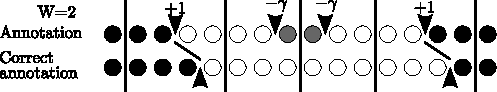
\includegraphics[width=10cm]{../figures/HERDbuddy.pdf}
\end{center}
\caption[Highest Expected Reward Decoding explanation]{
Triangles corresponds to the boundaries. Vertical lines corresponds to the windows
of size $2W$, or smaller to avoid overlaps. Windows around boundaries
represents regions where we search for the corresponding boundaries in the correct
annotation.
The first and the fourth boundary are correctly predicted because in the correct
annotation is boundary between same colors within distance $W=2$.
This picture was taken from \cite{Nanasi2010mgr}.
}\label{FIGURE:HERDBUDDY}
\end{figure}

We say that boundary on position $i$ is correctly predicted, if it satisfy
following conditions.
\begin{enumerate}[itemsep=-1mm]
\item There is boundary between same labels in the correct annotation on position $j$ and $j$ is
within distance $W$ from $i$ ($|i-j|\leq W$).
\item There is no other boundary between $i$ and $j$. 
\end{enumerate}
Boundaries are illustrated in figure \ref{FIGURE:HERDBUDDY}. 

Let $x$ be the number of correctly
predicted boundaries and $y$ be the number of other boundaries in the proposed
annotation. Then $f(\Lambda,\Lambda')=x-\gamma y$ where $\gamma$ is defined
constant. If $W=1$ then this is equivalent to the Maximum Boundary Accuracy
Decoding. Intuition behind this gain function is that we want to amplify the   
expected gain for the boundary if there are many annotations with similar
boundary.

Optimizing this criteria can be done in $O(|X|W|C||T| + n|C|^2W^2)$ time  and
$O(\sqrt{|X|}|C||V|+W|C||V|+n|C|^2)$ memory. Experimental evaluation,
optimization algorithm and implementation details can be found in
\cite{Nanasi2010,Nanasi2010mgr}.

\subsection{Distance Measures on Annotations}\label{SECTION:DISTANTMEASURES}

Another approach to solve similar problem was proposed by {\it Brown,
Truszkowski} in \cite{Brown2010}. Originally their implementation was aimed at
prediction of boundaries in transmembrane proteins \cite{Brown2010}, but later
they successfully adapted their algorithm to jumping HMMs \cite{Truszkowski2011}.
Their approach is trying to solve same problem as HERD: the exact boundaries of
an annotations are hard to find and grouping similar annotation is useful.
At first we give few definitions.

\begin{definition}
Let $d$ be any distance measure defined on annotations. Ball of radius $r$
around annotation $\Lambda$ is 
\begin{equation*}
B_d(\Lambda,r) = \{\Lambda'\mid d(\Lambda,\Lambda')\leq r\}
\end{equation*}
\end{definition}

\begin{definition}
Let $\Lambda=\Lambda_0\Lambda_1\dots\Lambda_{n-1}$ be an annotations. Footprint
of $\Lambda$ is maximal subsequence of $\Lambda$ that does not contain two
identical 
consecutive labels. \label{DEFINITION::FOOTPRINT}
\end{definition}

\begin{definition}
Let $b_i(\Lambda)$ be $i$-th boundary of $\Lambda$ and $b(\Lambda)$ be the
number of boundaries in $\Lambda$.
Border shift distance $d_{b}$ is 
\begin{equation*}
d_{b}(\Lambda,\Lambda') = \begin{cases}
\infty & \text{if $\Lambda$ and $\Lambda'$ have different footprint}\\
\max_{i=0}^{b(\Lambda)-1} d_i(\Lambda)-d_i(\Lambda') & \text{otherwise}
\end{cases}
\end{equation*}
and border shift sum distance $d_s$ is 
\begin{equation*}
d_{s}(\Lambda,\Lambda') = \begin{cases}
\infty & \text{if $\Lambda$ and $\Lambda'$ have different footprint}\\
\sum_{i=0}^{b(\Lambda)-1} d_i(\Lambda)-d_i(\Lambda') & \text{otherwise}
\end{cases}
\end{equation*}

\end{definition}

To predict the recombinations of sequences or the annotations of the
transmembrane proteins {\it Brown,
Truszkowski} maximize following function
\begin{equation*}
f_d(\Lambda,\Lambda') = 
\begin{cases}
1 & {\text if }\Lambda\in B_d(\Lambda',r)\\
0 & \text{otherwise}
\end{cases}
\end{equation*}

As distance $d$, they have considered Hamming distance, Border shift distance
and Border shift sum distance \cite{Brown2010}.  If we set $r=0$ then $f_d$ is
same as $f_A$ and therefore finding annotation that maximize $f_d$ is NP-hard.

Maximizing $f_d$ is NP-hard but finding the  annotation with footprint $F$ and
maximal expected gain can be done in polynomial time \cite{Brown2010}. Therefore
{\it Brown and Truszkowski} used following heuristic algorithm: At first 
sample the state paths to get the most probable footprint $F$ with high probability,
then use the
polynomial algorithm for finding the annotation with footprint $F$ and the highest expected gain.

Gain function $f_d$ is similar to $f_A$: the annotation is considered correct if
it is same/very similar to the correct one. MBAD, HERD and the
Posterior decoding do not care about overall structure of annotation, they
construct annotation from highly probable features. However,
decoding function $f_d$ take in to account
overall structure of the sequence.
